% Standalone TikZ source for the system architecture diagram.
% Build:  pdflatex architecture.tex  -->  architecture.pdf
% The compiled PDF is then included by main.tex via \includegraphics.
%
% Diagram blocks (per PAPER_NOTES.md "Figures needed" entry 1):
%   1. Data sources (5 ETF OHLCV)
%   2. MultiAssetTradingEnv state assembly
%        - per-asset OHLCV + indicators
%        - Phase-C liquidity-regime features (vol z-score, OHLC-disp spread)
%        - rolling 20-day correlation matrix (10 vals)
%        - position vector (5)
%        => 65/75-dim observation
%   3. Transformer encoder (causal self-attn, T=60, d=64, 2 layers, 4 heads)
%   4. x5 PPO heads (independent seeds, val-Sharpe early-stop)
%   5. Uncertainty-scaled aggregation: a = mu / (1 + beta * sigma_bar)
%   6. Kyle's-lambda market-impact cost + stochastic fill noise
%      -> reward signal back to env
%
% Annotate Phase-A (impact cost) and Phase-C (liquidity feats + fill noise)
% contributions distinctly (e.g. coloured borders or badge labels).

\documentclass[tikz,border=4pt]{standalone}
\usepackage{amsmath,amssymb}
\usepackage{tikz}
\usetikzlibrary{arrows.meta,positioning,shapes.geometric,fit,backgrounds,calc}

\begin{document}
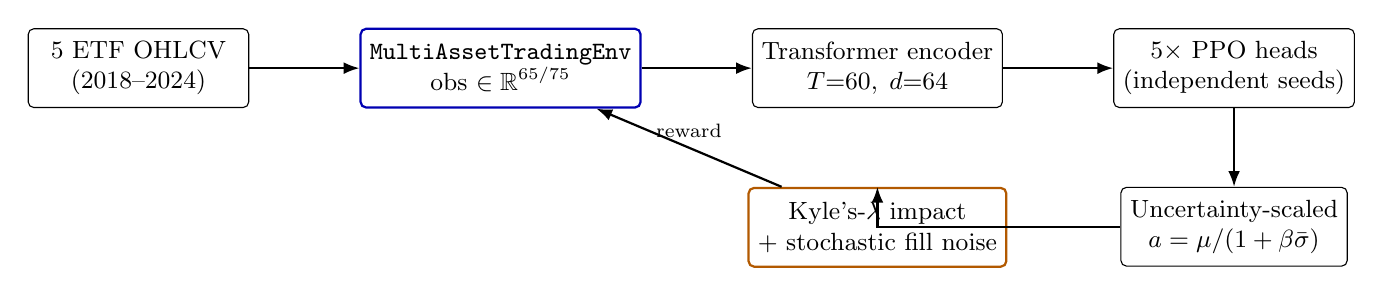
\begin{tikzpicture}[
  font=\small,
  node distance=10mm and 14mm,
  block/.style={rectangle, draw, rounded corners=2pt, align=center,
                minimum width=28mm, minimum height=10mm, fill=white},
  phaseA/.style={block, draw=orange!70!black, line width=0.8pt},
  phaseC/.style={block, draw=blue!70!black,   line width=0.8pt},
  arr/.style={-{Latex[length=2mm]}, thick},
]

% TODO (D18): flesh this out into the full pipeline. Below is a minimal
% three-block sketch that compiles standalone so the main paper has a
% buildable include path. Replace with the full 6-block diagram before
% paper submission.
\node[block]                       (data)  {5 ETF OHLCV\\(2018--2024)};
\node[phaseC, right=of data]       (env)   {\texttt{MultiAssetTradingEnv}\\
                                            obs $\in \mathbb{R}^{65/75}$};
\node[block, right=of env]         (xfm)   {Transformer encoder\\
                                            $T{=}60,\;d{=}64$};
\node[block, right=of xfm]         (heads) {$5\times$ PPO heads\\
                                            (independent seeds)};
\node[block, below=of heads]       (agg)   {Uncertainty-scaled\\
                                            $a = \mu / (1 + \beta\bar\sigma)$};
\node[phaseA, below=of xfm]        (cost)  {Kyle's-$\lambda$ impact\\
                                            $+$ stochastic fill noise};

\draw[arr] (data)  -- (env);
\draw[arr] (env)   -- (xfm);
\draw[arr] (xfm)   -- (heads);
\draw[arr] (heads) -- (agg);
\draw[arr] (agg)   -| (cost);
\draw[arr] (cost)  -- (env) node[midway, above, font=\scriptsize]{reward};

\end{tikzpicture}
\end{document}
